\chapter{Evaluation}
To ensure that the prototype satisfied our final problem statement, some evaluation had to be done on the prototypes performance. As described in the methods chapter (\ref{chp:methods}), the prototype would evaluated in two different tests. This chapter details how each of these were carried out. Results will be discussed in the following chapter.

\section{Expert usability evaluation}
It proved very difficult to find expert testers for the usability test. We took contact to 6 garden architects in the greater Copenhagen area and a few further away on Zealand the 1st of December. We sent a reminder on the 5th, as only one architect had responded. The responses from the experts were slow, and only arrived late in December. Due to concerns that we would be unable to get enough expert testers, we started a concurrent test on students at AAU CPH. It turned out that no experts were interested in testing the prototype, even though we were willing to travel great distances to test it. So all we were left with was the student usability test. This is not optimal in any way, but it is the way it turned out.
\section{Student usability test}
A student usability test was made to discover general usability problems. This was done by having non-members of the target group roleplay using the prototype as garden architects. Participants were gathered in groups of two, and would take turns being the architect and the "customer". Afterwards the architects would fill out a questionnaire from which the usability problems could be extracted. 
\subsection{Data gathering}
The main goal of the test was to find usability problems in the prototype. Speed was a factor, and for this reason we chose not to use the SUS questionnaire, unlike what we had planed to do with the architects. SUS only measures usability, but does nothing to explain the root causes of the usability problems. Often the SUS questionnaire will serve as the basis for a structured interview afterwards, where people can explain why they gave the marks they did. But this type of qualitative analysis is very time consuming to do. To get usability data fast, we devised a small questionnaire, presented in Appendix \ref{sec:appendixUsability}. The questionnaire would ask some Likert scale questions and some yes/no questions regarding if the participants had any problems using the prototype such as "were you able to do anything you and the client wanted" or "Did the program respond accurately to your actions". If they answered "no" the would be allowed to leave comments detailing why this was the case. Finally they were asked to rate the apparent advantages and disadvantages of the prototype compared to pen and paper.
\subsection{Sampling}
Due to the nature of the test participants were found using convenience sampling on AAU CPH.
\subsection{Test setup of the usability test.}
In Figure \ref{fig:test1}, the setup of the test can be seen.
\begin{figure}[H]
	\centering
	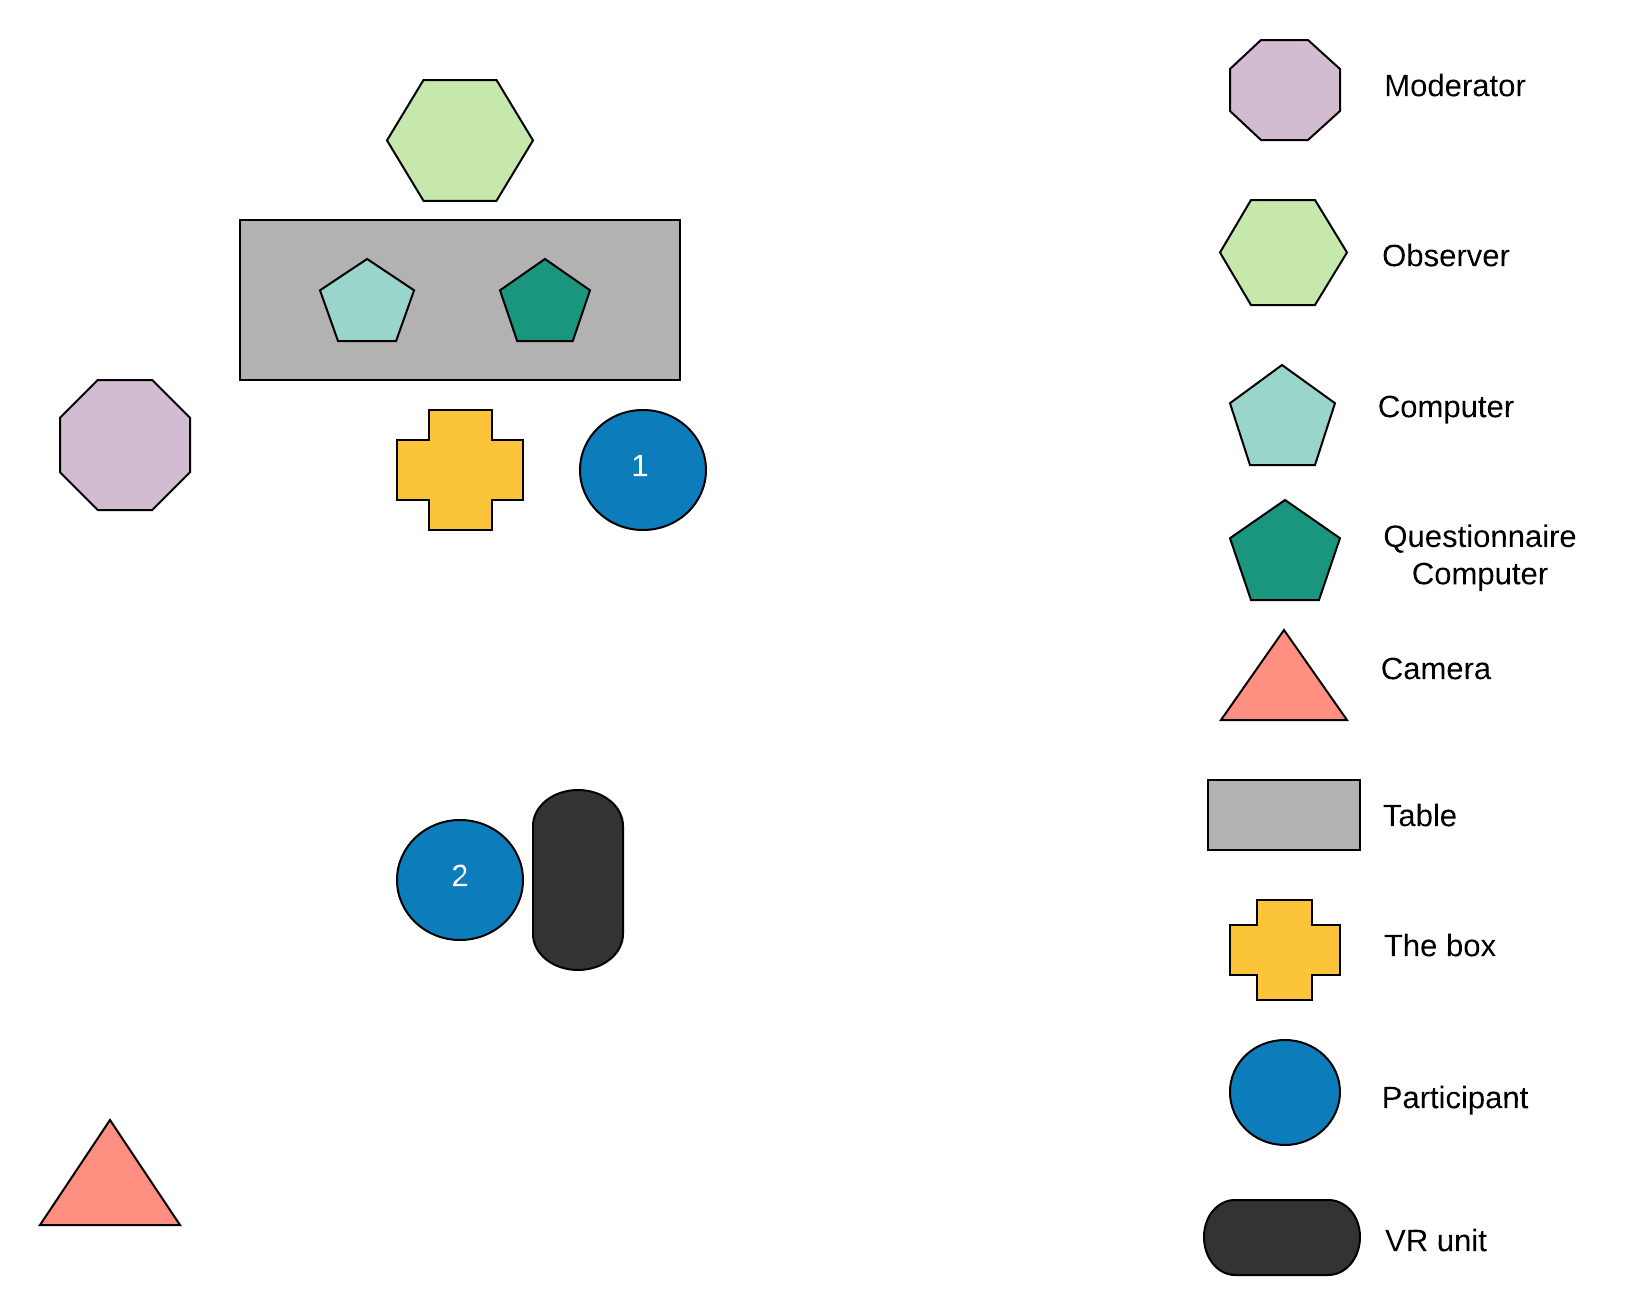
\includegraphics[width=1\linewidth]{figure/Evaluation/Test1.png}
	\caption{Our test setup, with the location of the participant, moderator, video camera and equipment. The two phases are visualized by the numbers in the circles.}
	\label{fig:test1}
\end{figure}

\subsection*{The equipment being used during the test}
\begin{itemize}
	\item[-] The box where the tokens is placed with a camera inside.
	\item[-] Laptop for filling out a questionnaire.
	\item[-] HTC vive VR unit.
	\item[-] Laptop with a GTX 1050 running the VR unit.
\end{itemize}
The laptop running the VR unit, are according to HTC's own minimum specification requirements, not powerful enough to run a virtual environment smoothly\footnote{\href{https://www.vive.com/us/ready/}{\color{blue}Vive recommended specifications for Virtual Reality}}.
\subsection*{Location and schedule}
The test took place Thursday 7/12 2017 in our group room at Aalborg University Copenhagen on Frederikskaj 12. Each testing with evaluation took approximately 15 to 20 minutes for two participants.

\subsection*{Test procedure}
Before the test began, the participants was informed about the general purpose of the test, tasks and their given consent to being recorded(for AVS production). After agreeing to this, the participants were asked to take the role of the customer or the architect. They where asked to role play planning and designing a new garden and find out what the design should look like. The client would take on the VR goggles and the architect would make a design with the markers, with the feedback from the client. After the participants tried their different roles the architect was asked to fill out the questionnaire (\ref{sec:appendixUsability})\todo{remove client questionnaire}. Afterwards the participants would switch roles and do the same thing again.
\subsection{Results}

\begin{figure}[H]
	\centering
	\begin{tikzpicture}
	\begin{axis}
	[
	boxplot/draw direction=x,
	height=5cm,
	width=8cm,
	enlargelimits=0.03,
	xtick={1,1.5,2,2.5,3,3.5,4,4.5,5},
	ylabel=,
	xlabel={Agreement to how easy the product was to use?},
	yticklabels={}
	]
	\addplot+[boxplot]
	table[row sep=\\,y index=0] {
		data\\ 1\\ 3\\ 3\\ 4\\ 4\\ 5\\ 5\\ 5\\
	};
		
	\end{axis}
	\end{tikzpicture}
	\caption{Box plot graph showing the results of the architect scale questions.}
	\label{fig:boxPlotResults2}
\end{figure}

\subsection*{Was the framerate (the frequency at which the screen updates) tolerable?}
As seen in \autoref{fig:barChartFrame}, 3 of the 8 participants didn't find the framerate very tolerable. 1 participant found it somewhat tolerable and 3 participants found it very tolerable.

\begin{figure}[H]
	\centering
	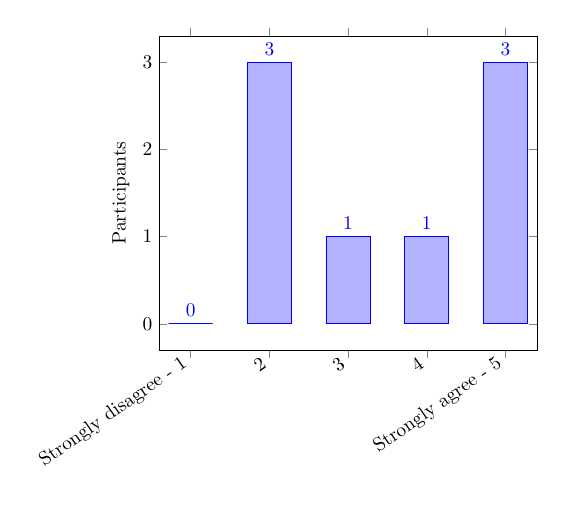
\begin{tikzpicture}[scale=0.7]
	\begin{axis}[ybar,bar width=0.8cm,enlargelimits=0.1,legend style={at={(0.5,-0.2)},anchor=north,legend columns=-1},ylabel={Participants},symbolic x coords={Strongly disagree - 1,2,3,4,Strongly agree - 5},xtick=data,nodes near coords,nodes near coords align={vertical},x tick label style={rotate=35,anchor=east},]
	\addplot coordinates {(Strongly disagree - 1,0) (2,3) (3,1) (4,1) (Strongly agree - 5,3)};
	\end{axis}
		
	\end{tikzpicture}
	\caption{Bar chart showing if the participants found the framerate tolerable.}
	\label{fig:barChartFrame}
\end{figure}

\subsection*{How easy was the product to use?}
Out of 8 participants 1 of them strongly disagreed that the product was easy to use, while 2 participants hit the middle ground and 5 participants agreed that the product was easy to use. This can be seen in \autoref{fig:barChartEasy}.

\begin{figure}[H]
	\centering
	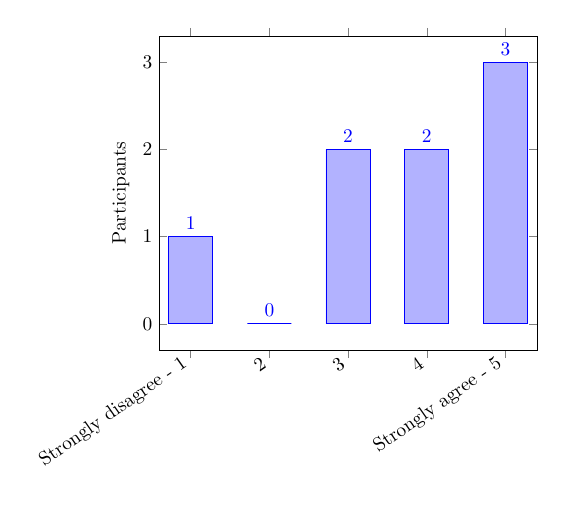
\begin{tikzpicture}[scale=0.7]
	\begin{axis}[ybar,bar width=0.8cm,enlargelimits=0.1,legend style={at={(0.5,-0.2)},anchor=north,legend columns=-1},ylabel={Participants},symbolic x coords={Strongly disagree - 1,2,3,4,Strongly agree - 5},xtick=data,nodes near coords,nodes near coords align={vertical},x tick label style={rotate=35,anchor=east},]
	\addplot coordinates {(Strongly disagree - 1,1) (2,0) (3,2) (4,2) (Strongly agree - 5,3)};
	\end{axis}
	
	\end{tikzpicture}
	\caption{Bar chart showing if the product was easy to use.}
	\label{fig:barChartEasy}
\end{figure}
\subsection{Usability feedback questions}
Some of the questions in the questionnaire were yes no questions that dealt with usability very broadly, if the participant answered no to these questions they were able to leave comments explaining why. The questions and response rates can be seen in Figure \ref{fig:pie1} and \ref{fig:pie2}.
\begin{figure}[H]
	\centering
	\begin{minipage}[b]{0.49\textwidth}
		\begin{figure}[H]
			\centering
		\textbf{	Were you able to do everything you and the client wanted?}
			\begin{tikzpicture}
			\raisebox{-8pt}{
			\pie [sum=auto,text=inside,before number =,after 		number=,rotate=0,radius=2,color={red!50 , black!20},explode=0.1]
			{3/No, 5/Yes}
			}
			\end{tikzpicture}
			\caption{Pie chart showing visualizing whether or not the participants (n=8) were able to do everything that the client wanted.}
			\label{fig:pie1}
		\end{figure}
	\end{minipage}
	\hfill
	\begin{minipage}[b]{0.49\textwidth}
		\begin{figure}[H]
			\centering
			\textbf{	Did the prototype respond accurately to your actions?}
			\begin{tikzpicture}
			\raisebox{-8pt}{
				\pie [sum=auto,text=inside,before number =,after 		number=,rotate=0,radius=2,color={red!50 , black!20},explode=0.1]
				{4/No, 4/Yes}
			}
			\end{tikzpicture}
			\caption{Pie chart showing visualizing if the participants (n=8) thought the program responded accurately to their actions.}
			\label{fig:pie2}
		\end{figure}
	\end{minipage}
\end{figure}
This data in itself is not very interesting for us. But the comments left by the participants were. A few usability problems became clear even from the small number of test that were conducted.

\subsection*{Orientation of markers in relation to the world}
The top of the tokens have a rendered picture of the object the represent(see Section \ref{sec:tokentop}). However this gives no overview of the direction the object will be facing inside the vr. One participant commented.  
\\
\begin{quote}
\textit{i was not really sure about where the client was in the scene and his orientation. The tokens show an image so I tried to use it to help me with the orientation\\}
\end{quote}
This is a big problem when trying to correctly place objects where the direction is important, like a bench. Placing benches looked over a pool was a problem for instance. One solution to change the top of the tokens, to display the object from a top down view, which is the view of the architect. Another could be to add a feature to the top that would enable architects to see the direction clearly.

\subsection*{Orientation of client in relation to tokens}
The architect had no way of knowing where the customer were in relation to the garden he/she was building. This sometimes made communication between the two very difficult. The customer would point an object, an ask that it be moved a bit to the right, and the architect would have no idea which object it was, and which way the customers right was. Testers commented\\
\begin{quote}
	\textit{Was hard to place objects since i had difficulty with where they would appear compared to the client\\}
\end{quote}

\begin{quote}
	\textit{I had a hard time knowing where the client was on the glass plate compared to the items. Sometimes there were some consistency in where i placed the item and where it appeared, but i got the hang of it eventually\\}
\end{quote}

\begin{quote}
	\textit{orientation is very difficult to understand\\}
\end{quote}
 Allowing the customer to  highlighting objects in a way that could be displayed to the client would greatly reduce miscommunication. Furthermore, showing on the plate where customers was at the moment would greatly help with understanding their requests. Another way would be to introduce a "client" token that would control the clients position. This would allow architects to take the customer on a guided tour through out the garden.
\subsection*{Were you able to do everything you and the client wanted?}
As seen in \autoref{fig:pie1} over half of the participants answered yes to this question, and a little under half of them answered no.

If the participant answered no, they had the ability to clarify further, such two comments were:\\

 \begin{quote}
 	
\textit{I had a hard time knowing where the client was on the glass plate compared to the items. Sometimes there were some consistency in where I placed the item and where it appeared, but I got the hang of it eventually}\\
  \end{quote}
  
\begin{quote}
\textit{Orientation is very difficult to understand}\\
\end{quote}	
 	 
As it can be seen from the given answers, some of the participants had a hard time figuring out where the client was in the garden, which made it difficult for them to know where to place the objects in regards to the client.


\subsection{Findings}
A fair amount of participants answered that they were able to do what the clients wanted as seen in \ref{fig:pie1}. A common statement from the participants was that it was difficult for them to localize the client in the garden. The architect couldn't see where the client was in the garden, because the client was able to move around freely inside the VR garden.\\

Over half of the participants answered that it was easy to follow the clients' instructions (see \autoref{fig:pie2}). Because we did not use a follow up question for this question we can't directly say why the last segment of participants had difficulties following the clients instructions.\\



\section{Immersion test}
The immersion test was conducted to test how immersive our prototype was compared to two of the tools traditionally employed by garden architects, sketching and a 3D fly through. From the analysis in section \ref{sec:immersion} it was found that immersive virtual reality resulted in better spacial perception. As such, if our prototype feels more immersive it might be a better tool for presenting designs to clients.

\subsection{Test goals}
The goal of the test was to determine if the prototype in fact did answer the final problem statement (\autoref{sec:FPS}). The keywords from the FPS are:
\begin{itemize}
	\item[-] Fast
	\item[-] Efficient
	\item[-] Immersive
\end{itemize}
as such we were keen on measuring these goals in this test.
\subsection{Sampling}
Finding real garden architects among the students at AAU CPH, turned out to be a big challenge, and therefore it was decided that convenience sampling were to replace that criteria. Convenience sampling among the students at AAU CPH gave us 12 test participants in total.
\subsection{Environment}
The test were carried out in our group room. The group members who were not part of the test would leave and work elsewhere during testing period. This was very much an artificial environment, again due to the difficulty getting a hold of target group members. The artificial environment allowed to do large quantities of tests, as we could bring participants into highly controlled situation and test very specific elements of the experience.\cite[p.~64]{bjoernerBog}
\subsection{Test specifics}
The participants were told they would be trying three different technologies, and were asked to try and understand the layout, in such a way that they could visualize it themselves. The participant were told to take as long as they needed with each of the parts. The parts consisted of:
\begin{itemize}
	\item[-] 2D sketching
	\item[-] 3D viewing
	\item[-] Virtual reality
\end{itemize}
After each part a four question questionnaire of Likert scales was filled out. The results from it can be seen in Appendix \ref{sec:appendixImmersionTest}. This meant that each person would answer the same questionnaire three times. From this we would be able to see how the testers rated the different parts in terms of immersiveness, speediness of spacial understanding, perceived usefulness to garden architects, and understanding of the gardens design. To differentiate between the subjects they were each given a participant number. As each participant spend longer time observing the garden, we predicted their understanding would improve. To eliminate this bias we used every possible sequence combination of 2D sketching, 3D viewing and Virtual Reality on two differently designed gardens, as seen in \autoref{table:immersionCombinations}.

\begin{table}[H]
	\centering
	\caption{All the sequence combinations of 2D sketching, 3D viewing and virtual reality, and which participant that did what combination.}
	\label{table:immersionCombinations}
	\begin{tabular}{l | c|c|c|c|c|c}
		&
		\begin{tabular}[c]{@{}c@{}}VR\\ 2D\\ 3D\end{tabular} & \begin{tabular}[c]{@{}c@{}}VR\\ 3D\\ 2D\end{tabular} & \begin{tabular}[c]{@{}c@{}}2D\\ 3D\\ VR\end{tabular} & \begin{tabular}[c]{@{}c@{}}2D\\ VR\\ 3D\end{tabular} & \begin{tabular}[c]{@{}c@{}}3D\\ VR\\ 2D\end{tabular} & \begin{tabular}[c]{@{}c@{}}3D\\ 2D\\ VR\end{tabular} \\ \hline 
		Garden 1 & 2                                                                            & 5                                                                            & 4                                                                            & 3                                                                            & 1                                                                            & 6                                                                            \\ 
		Garden 2 & 7                                                                            & 8                                                                            & 9                                                                            & 10                                                                           & 11                                                                           & 12                                                                           \\
	\end{tabular}
	
\end{table}
The 2D sketches the participants were asked to study can be seen in \autoref{fig:sketchGarden1} and \autoref{fig:sketchGarden2}. These were both created from the 3D virtual scenes made in Unity. The two gardens purposely have two very different layouts, and two very different complexity levels(The number of objects in the scene). This was done in an attempt to eliminate bias and the odds of the results being up to chance, as one layout might favor one part.
\begin{figure}[H]
	\centering
	\begin{minipage}[b]{0.49\textwidth}
	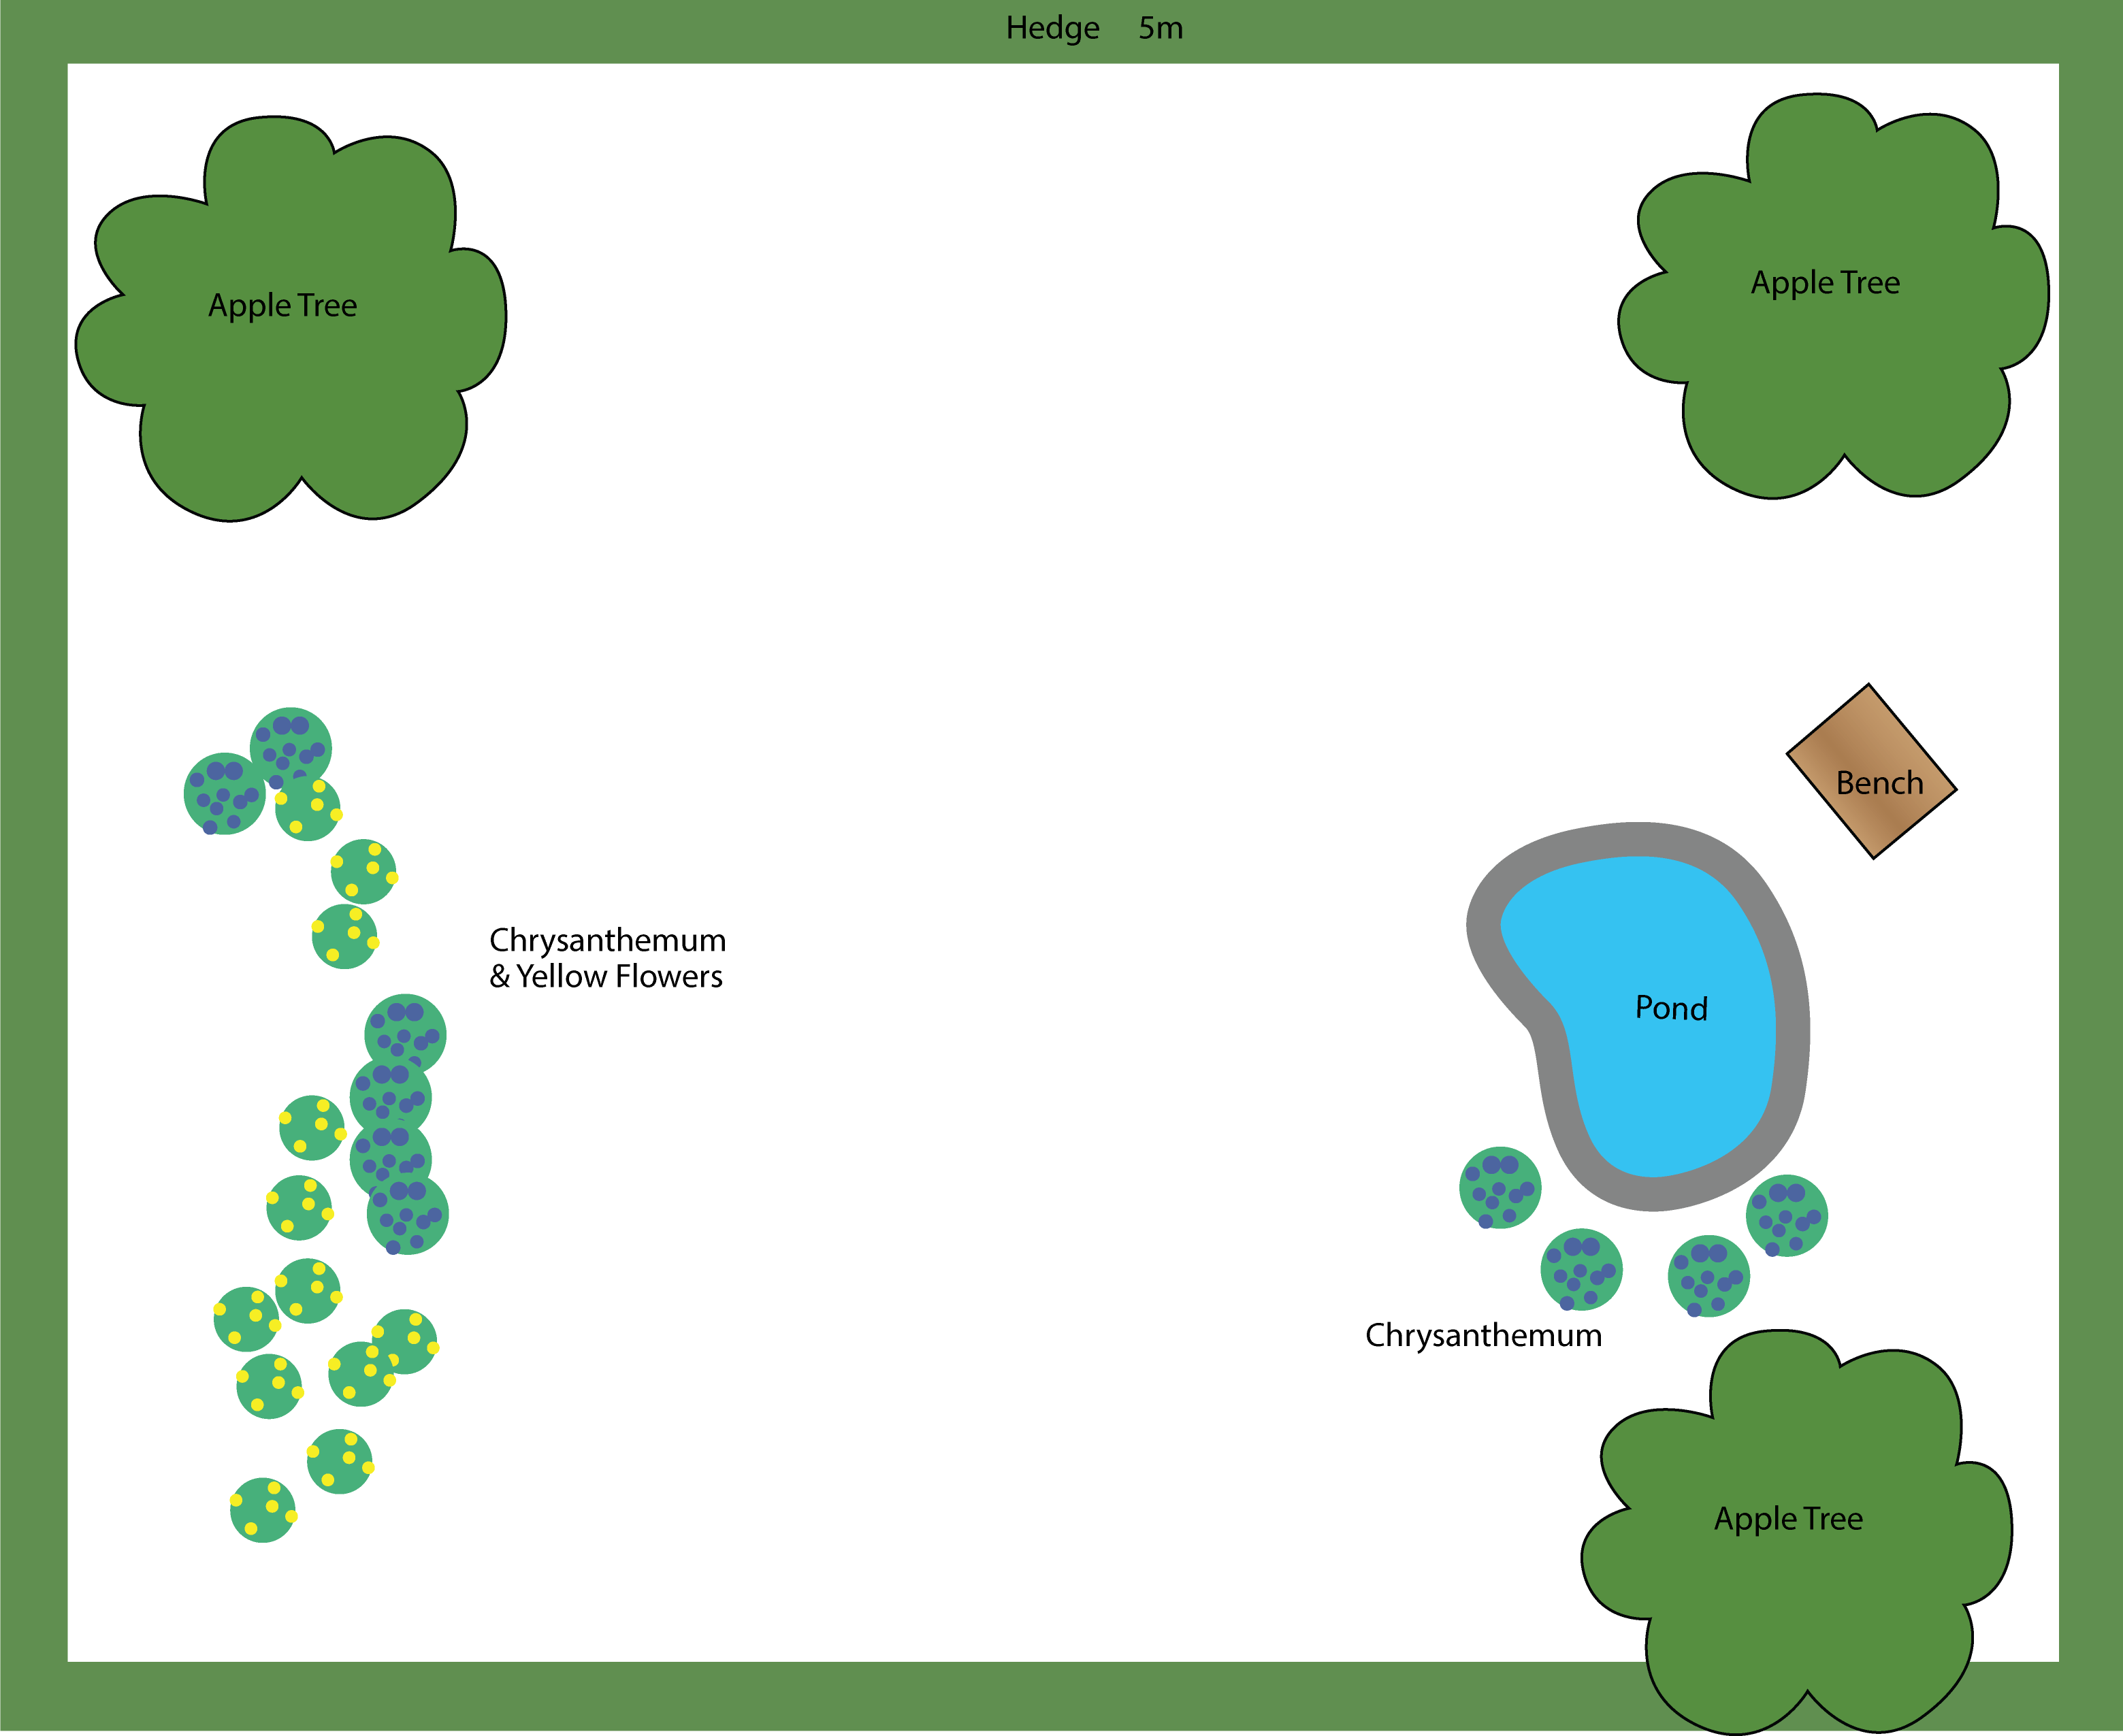
\includegraphics[width=1.0\linewidth]{figure/Evaluation/Garden1.png}
	\caption{Sketch garden 1}
	\label{fig:sketchGarden1}
	\end{minipage}
	\hfill
	\begin{minipage}[b]{0.49\textwidth}
	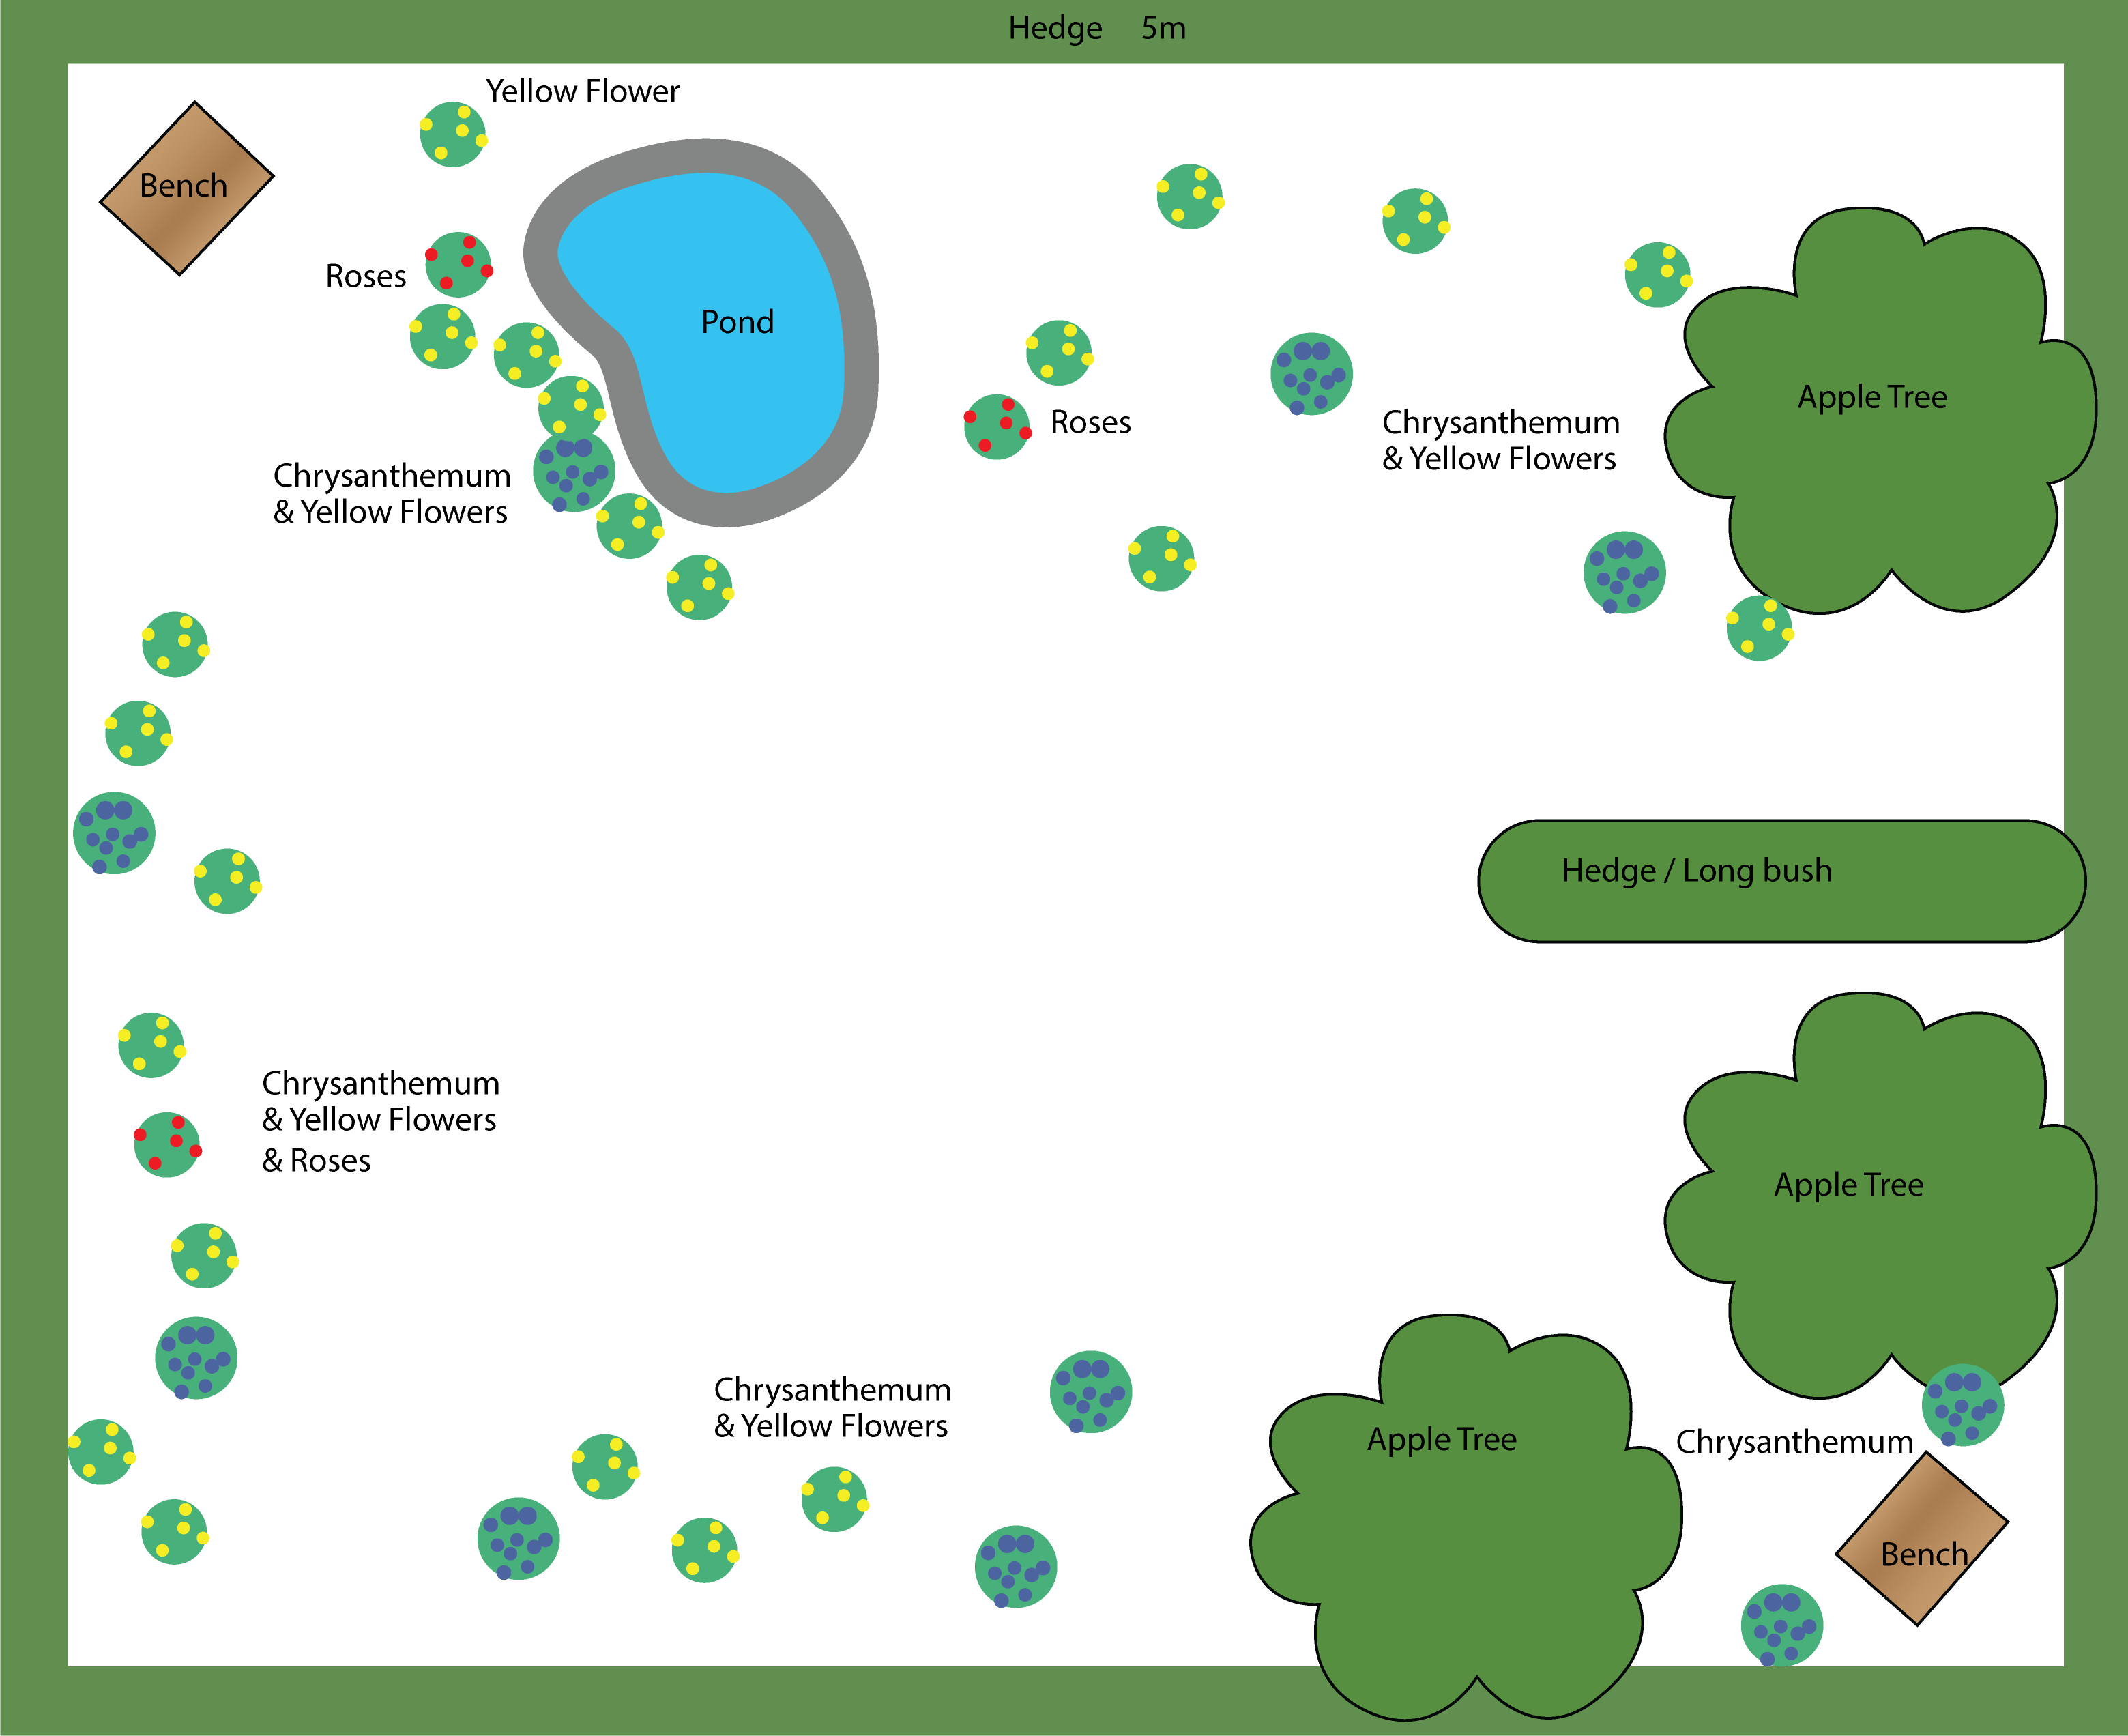
\includegraphics[width=1.0\linewidth]{figure/Evaluation/Garden2.png}
	\caption{Sketch garden 2}
	\label{fig:sketchGarden2}
	\end{minipage}
\end{figure}
The 3D scenes had a camera that automatically moved and looked around the garden. This was done to replicate what we observed some garden architects were advertising on their web pages\footnote{Visualization done by garden architect : \url{https://youtu.be/1ki9H5fs7EI}}. In VR, the participants could use the controller to teleport around and observe the garden, as described in Section \ref{sec:designUI}. 

\subsection{Findings}
After the tests had finished, we compiled the answers into two tables, one for garden 1 (\autoref{table:averageResponseGarden1}) and one for garden 2 (\autoref{table:averageResponseGarden2}). These tables contained the averages of the responses.
\begin{table}[H]
	\centering
	\caption{Average of responses with test on garden 1, higher numbers are better}
	\label{table:averageResponseGarden1}
	\begin{tabular}{p{3cm}|p{3cm}|p{2cm}|p{3cm}|p{3cm}}
		Test type       & How long do you think it took you to gain insight into how it would be, to be in the garden? (1-10) & How immersed did you feel? (1-10) & How useful do you think this tool could be for a garden architect? (1-5) & How much do you feel like you understood the garden's design? (1-10) \\ \hline
		&&&&\\
		Sketching       & 6.75    & 2.00    & 3.92      & 7.58            \\
		3D Viewing      & 6.08  & 4.67  & 4.00    & 8.67               \\
		Virtual Reality & 8.17     & 7.67     & 4.58      & 9.17    
	\end{tabular}
\end{table}
From \autoref{table:averageResponseGarden1} it can be be seen that for all four questions, Virtual reality was rated higher than when 3D viewing and 2D sketching. For the first question, about the length of time it took the participant to gain insight into how it would be, to be in the garden, in both garden 1 and 2, the participants rated virtual reality as the quickest (Higher number is faster). In both gardens however, the 3D viewing experience was rated the slowest (6.08 and 5.50).
\begin{table}[H]
	\centering
	\caption{Average of the responses with test on garden 2, higher numbers are better}
	\label{table:averageResponseGarden2}
	\begin{tabular}{p{3cm}|p{3cm}|p{2cm}|p{3cm}|p{3cm}}
		Test type       & How long do you think it took you to gain insight into how it would be, to be in the garden? (1-10) & How immersed did you feel? (1-10) & How useful do you think this tool could be for a garden architect? (1-5) & How much do you feel like you understood the garden's design? (1-10) \\ \hline
		&&&&\\
		Sketching       & 7.00                                                                                         & 2.33                       & 4.00                                                               & 8.00                                                          \\
		3D Viewing      & 5.50                                                                                         & 4.67                       & 3.83                                                               & 7.83                                                          \\
		
		Virtual Reality & 8.00                                                                                         & 6.17                       & 4.50                                                               & 8.67                                                         
	\end{tabular}
\end{table}

In general, when asked about how immersed the participants felt during the test, they picked much higher numbers in garden 1 than garden 2, we believe this to be down to the difference in complexity between the two gardens, as garden 2 have substantially more objects in the scene, and is therefore more complex to understand.
The question about immersiveness was on a scale from 1 to 10, and generally 2D sketching wasn't making the participants feel immersed, while Virtual reality on the other hand, in garden 1, was almost ranked 4 times higher.\\

Usefulness was rated on a scale on from 1 to 5, and overall usefulness is rated high, with the lowest average being 3D viewing in garden 2, rated at 3.83. This question was designed to make the participant take the standpoint of a garden architect, and hence try to visualize the usefulness of each tool in the hypothetical work flow.\\
To better get an idea of whether or not the participant could understand the garden they were seeing, they were asked to rate their own understanding of the garden's design on a scale from 1 to 10. Just like the usefulness response, all of the answers were quite high, with the lowest being 7.58, for sketching in garden 1.\\

All but 1 participant answered the final question prompting a comparison between the three different mediums. 
The contents of the comments have been separated into statements about the individual mediums:
\subsection*{3D viewing}
	8 out of 12 participants left a comment on what could be changed for 3D viewing. Of those, 7 comments concerned the ability to navigate or interact with the environment themselves. One comment said it would be beneficial to see the dimensions of the objects in the garden. A list of the condensed comments in in descending order can be seen in \autoref{table:condensed3D}.
		\begin{table}[H]
		\centering
		\caption{Comments about the 3D viewing, condensed into categorized statements}
		\label{table:condensed3D}
		\begin{tabular}{p{5cm}|c}
			Comment & Count \\ \hline
			Bad to not have control & 3 \\
			Some immersion & 3 \\
			Fast overview &2 \\
			Lacking some immersion &2 \\
			Felt polished& 1 \\
			Lack of dimensions& 1 \\
			Good for angles& 1 \\
			Lack of depth perception& 1 \\
			Movement confusing& 1 \\
			Strange& 1 \\
			Good idea of layout& 1 \\
		\end{tabular}
	\end{table}
\subsection*{2D Sketching}
	Of the sketching comments, 9 of 12 testers left a comment. Five comments said they wouldn't change anything or didn't know what they'd change. Two comments said they needed more depth to the image. One tester wanted a more detailed sketch, and one asked for a "more immersive experience" The tester who left the last comment started with the 2D sketch as the first medium for visualization and may have found the immersion question silly without any other medium to compare it to. A list of the condensed comments in descending order can be seen in \autoref{table:condensed2D}.
	\begin{table}[H]
		\centering
		\caption{Comments about the 2D sketching, condensed into categorized statements}
		\label{table:condensed2D}
		\begin{tabular}{p{5cm}|c}
			Comment & Count \\ \hline
			Quick & 3 \\
			Descriptive & 2\\
			Not immersive & 2 \\
			Good for accurate positions & 2 \\
			Good overview  & 2 \\
			Easy to understand & 2 \\
			Difficult to visualize & 1 \\
			Inaccurate& 1 \\
			Good for sizes & 1 \\
		\end{tabular}
	\end{table}
\subsection*{Virtual Reality}
	As for the Virtual Reality test, 9 out of 12 testers left a comment. A list of the condensed comments in descending order can be seen in \autoref{table:condensedVR}.
	\begin{table}[H]
		\centering
		\caption{Comments about the virtual reality, condensed into categorized statements}
		\label{table:condensedVR}
		\begin{tabular}{p{5cm}|c}
			Comment & Count \\ \hline
			Good for immersion & 7 \\
			Good feel of garden & 4 \\
			Good for size  & 2 \\
			Useful & 2 \\
			Lacking interactivity & 2 \\
			Good for angles & 1 \\
			Good for distances& 1 \\
			Lack of dimensions& 1 \\
			Good for focus on detail& 1 \\
			Limited FOV& 1 \\
			Natural& 1 \\
			Interesting& 1 \\
			Quick insight& 1 \\
			Low FPS& 1 \\
			Lack of overview& 1 \\
			Good for layout& 1 \\
			
		\end{tabular}
		
	\end{table}
 1 of the 9 didn't know what could be improved. 1 person wanted elements like floor plans. Two wanted improved graphics. One person wanted a note taking functionality, the ability to highlight objects, and multi-user functionality. Two users wanted more interactivity, and two users wanted a larger area to walk around in, as to remove the need for teleportation.\\\\

The tests proved that virtual reality has some immersion benefits over sketching on a piece of paper and a 3D camera flyby, and that participants felt that they understood the garden design better with Virtual Reality.
